\chapter{Integration of Transcriptomic with Proteomic data}\label{ch:Integration}
\setlength{\epigraphwidth}{0.8\textwidth}
\setlength{\epigraphrule}{0pt}
\epigraphhead[5]{%
\epigraph{\emph{Scientists like ripping problems apart, collecting as much data as possible\\
and then assembling the parts back together to make a decision.}}{Shirley M. Tilghman}
}

\vspace{2cm}
After assessing the similarity of the human gene expression profiles
across various tissues
at transcriptomic level (with \Rnaseq\ studies in \Cref{ch:Transcriptomics})
and proteomic level (with \emph{bottom-up} \ms\ studies in \Cref{ch:proteomics}),
my next step is to examine how these gene expression profiles
compare between these two different biological layers.\mybr\

One major aim of this study is to asses
how the correlations between the transcriptome and proteome
described in the literature, mostly measured in cells,
hold at the tissue level.
Moreover, good correlations may potentially lead to
the development of new strategies.
These may use the expression levels of \mRNA\ as proxies
to estimate protein expression,
which is generally difficult to measure directly (see \Cref{sec:exploreProtMS}).\mybr\

I have performed the integration and all the analyses presented in this chapter
under the supervision of \alvis\ and \jyoti.
A manuscript describing this work
and the new method of protein quantification, presented in \Cref{sec:NewQuantProt},
is in preparation.\mybr\

A few closely related studies~\mycite{SciRep2016,Franks2017-bp,Wang2019-ut} have
been published while I was working on
the integration of the non-diseased human transcriptome and proteome.
As their analyses rely on the same data sets (\ie\ \uhlen, \gtex, \pandey\ Lab data)
that I include in my work,
I describe and discuss together my results and theirs
whenever relevant.\mybr\

\clearpage
\derivativeWork{}
\begin{itemize}[topsep=0pt,nosep]
    \item (poster) CSHL  Biology of Genomes 2015 --- A feasibility study:
        Integration of independent human \Rnaseq\ and proteomic datasets
    \item (submitted paper) Mitra P. Barzine, K\={a}rlis Freivalds, James Wemright et al. (2020).
        Using Deep Learning to Extrapolate Protein Expression Measurements.
    \item (submitted paper) Andrew F. Jarnuczak; Hanna Najgebauer; Mitra Barzine;
        Deepti J. Kundu; Fatemeh Ghavidel; Yasset Perez-Riverol; Irene Papatheodorou; Alvis Brazma;
        Juan Antonio Vizcaíno An integrated landscape of protein expression in human cancer
    \item (talk) \gtex\ meeting 2017 --- A. Brazma Correlating transcriptome
        and proteome in human tissues
    \item (poster) HUPO 2018 --- Jarnuczak \etal\ An integrated atlas of
        protein expression in human cancer derived from publicly available
    \item (poster) ECCB 2018 --- Viksna \etal\ An integrated approach
        to missing data imputation in quantitative proteomics experiments
    \item (poster) RECOMB 2018 --- Viksna \etal\ Deep learning
        for protein abundance prediction using Gene Ontology and RNA abundance information
\end{itemize}

\clearpage\

%\vspace{-1cm}

An on-going debate in the literature is
whether good correlations of expression levels prevail
between \mRNAs\ and proteins \mycite{Uhlen:2016}.
The implicit assumption of a proportional relationship is persisting
as the many remaining technological limitations prevent
rigorous testing \mycite{Vogel2012-sq}.
To date, the existence or concentration of a given \mRNA\ transcript
is usually insufficient to ensure detection of the protein in a sample.\mybr\

On the one hand,
\citet{Ramakrishnan2009-lv} report that
\mRNAs\ abundance are roughly sufficient to predict
the protein presence or absence from a sample and
\citet{Vogel2010-ux} that
\mRNA\ level estimations and sequence features are enough to predict
two-thirds of the human protein abundance variation.\mybr\

On the other hand,
the literature fails to report any high correlation
between the transcriptome and the proteome for any organism.
Previous investigations found low or no correlation
between the measured expression profiles of the \mRNAs\ and
proteins in human~\mycite{Anderson1997-le,Chen2002-ob,Tian2004-hh,Pascal2008-gh,%
Gry2009-zv,Lundberg2010-gk},
other mammals~\mycite{Ghazalpour2011-nb},
and across many other species~\mycite{Gygi1999-fl,Maier2009-pb,Maier2011-tz,%
Yeung2011-sl,Palmblad2013-ji,Freiberg2016-fu}.\mybr\

In their encompassing reference experiment,
Schwanhäusser \etal{}~\mycite{schwanhausserglobal:2011,Schwanhausser2013-et}
present rather moderate correlations ($r^2≤0.41,\ie~r<0.64$)
and highlight that \mRNA\ levels explain only about 40\% of protein variations
they have observed.\mybr\

Other studies have explored the \mRNAs\ and proteins relationship in answer
to stimuli~\mycite{Marguerat2012-sn}
or with an increased focus to post-transcriptional regulations
(including degradation rates)~\mycite{Jovanovic2015-wv}.
While many other regulatory processes may occur
(\eg\ translation rates),
post-transcriptional modifications and technical noise
are (still) perceived as the probable primary sources
of \mRNA/protein concentration discrepancies~\mycite{Vogel2012-sq,Plotkin2010-ug}.\mybr\

Joint studies of transcriptome and proteome have already helped to highlight
links between genotype and phenotype~\mycite{Vogel2012-sq}.
However, the mitigated results reported above may explain
the focus shift of many subsequent studies.
While previous efforts were about linking the actual expression levels,
more recent studies primarily have mostly compared qualitative attributes
of given proteins and related \mRNAs{}.
Examples include the comparison of
the presence or absence of \mRNAs\ and their proteins
in specific conditions or tissues~\mycite{Santos2015-rj,Freiberg2016-fu,Uhlen2015}
or the comparison of their differential expression profiles
across identical sets of conditions~\mycite{Varemo2015-uk}.\mybr\

All (or almost all) aforementioned studies have turned to cells
for their joint analyses of transcriptome and proteome.
In contrast,
the analyses and integration I present in this chapter are
based on tissue studies.\mybr\

%\vspace{-2mm}
\section{Data~and~principal~analytical~approaches}\label{sec:IntegrationData}
%\vspace{-4mm}
Since the human proteome drafts~\mycite{PandeyData,KusterData} in 2014,
we have an unparalleled availability of large-scale tissue studies
both at the transcriptomic and proteomic layers to explore and integrate together
(see \Cref{ch:datasets}).
While these data are independent
(collected from various individuals, prepared,
and characterised by different laboratories),
their combined study may help
to shed light on the relationship
between the transcriptome and proteome at the tissue level.
Using different sources for the transcriptome and proteome
increases the overall technical noise,
but it may also help to highlight relevant biological signals (as
they need to be stronger than the noise and batch effects to be captured).\mybr\

In \Cref{ch:Transcriptomics}, I show that
the transcriptome \Rnaseq\ datasets present high interstudy tissue correlations
(median value for Pearson: $r_{\setOneMath}=0.75$; $r_{\setTwoMath}=0.85$ ---
Spearman: $\rho_{\setOneMath}=0.88$; $\rho_{\setTwoMath}=0.93$).
For this chapter analyses,
I only consider the datasets with the highest similarity
(highest correlations)
that incidentally comprise the greatest number of tissues
and are the two most recent studies,
\ie\ \dataset{Uhlén \etal}~\mycite{Uhlen2015}
and \gtex{}~\mycite{GTExTranscript} data.\mybr\

To compensate for the shortfalls in the study design implied
by the reuse of published data\footnote{%
Independent data also means
different collection and sampling processing methods and
lack of information on the samples population background.},
I use both \uhlen\ \etal\ and \gtex\ data
to filter out \mRNAs\ with high interstudy variability for identical tissues.
Whether this variability is technical or biological is irrelevant;
in both cases,
interpreting the relationship
between a highly variable \mRNAs\ and its protein from another dataset
remains hard to interpret.
For these \mRNAs,
it is impossible to explain the observed variability
between the two transcriptomic datasets.
Indeed, any result is subject to the transcriptomic dataset chosen
for the comparison with the proteomic one.
Furthermore, the comparison of the two transcriptomic data may give a reference,
\ie\ an ideal case scenario, for the proteomic/transcriptomic one.\mybr\

On the other hand,
as shown in \Cref{subsec:protTechVarHigh},
the technical variability prevails over
the biological signal of same-tissue samples
for the available high-throughput proteomics.
With the current technological state,
different tissues from the same proteomic study are more likely
to present a higher correlation
than the same tissues from two different studies.\mybr\

To avoid an overly restricted protein set for the following analyses,
I only include one proteomic study: \pandey\ Lab~\mycite{PandeyData}.
All its samples have been run through the same \ms\ platform and
with the same protocol.
Moreover, it presents more homogeneous protein distributions
(see \Cref{fig:distribProt} and \Cref{fig:pandeyDistribQ1Q2}) and
quantifies more proteins per tissue (\Cref{fig:distribProtUniq3D})
than the two other datasets.
Since a current major limitation of bottom-up \ms\ proteomic studies
is the possible lack of detection of proteins for various reasons
(see \Cref{subsec:simpleProt}),
the higher number of detected proteins in \pandey\ Lab data suggests that
this dataset has a higher quality than the two others.\mybr\

%Many strategies are recommended to increase the depth of the coverage
%(\eg\ \mycite{Zhang2014,Eriksson2007-si,Koziol2013-si}).
%Put together, these facts suggest that
%the \pandey\ Lab data has a higher quality than the two other datasets.
%\vspace{-0.5mm}

Though I include one proteomic dataset only,
as the literature reports that
the proteome is more conserved than the transcriptome
(across individuals and species)~\mycite{Laurent2010-rg,Liu2016-re},
this data collection ought to provide
a crude estimate of the extent of observations
that hold from cell to tissue level.\mybr\

This chapter integrates and analyses the matching pairs of \mRNA/proteins
of the common set of tissues between \pandey\ Lab
and the two transcriptomic datasets.\mybr\

\subsection{Overlapping set of tissues for the three datasets}

\begin{figure}[!htbp]
    \includegraphics[scale=0.69]{integration/PandeyGtexUhlen_tissuesVennm.pdf}
    \centering
    \caption[Number of shared and unique tissues between the proteomic
    dataset from Pandey Lab and the transcriptomic datasets (Uhlén \etal\ and
    Gtex)]{\label{fig:VennTissuePandeyGtexUhlen}\textbf{Number of shared and unique
    tissues between the proteomic (Pandey Lab) and the
    transcriptomic (Uhlén \etal\ and GTEx) data.} %The twelve common tissues of
    %the three datasets are
    %\tissue{Adrenal gland}, \tissue{Bladder}, \tissue{Colon}, \tissue{Oesophagus},
    %\tissue{Heart}, \tissue{Kidney}, \tissue{Liver}, \tissue{Lung}, \tissue{Ovary},
    %\tissue{Pancreas}, \tissue{Prostate} and \tissue{Testis}. The three added
    %tissue between \dataset{Uhlén \etal} and \dataset{Pandey Lab} are
    %\tissue{Gall bladder}, \tissue{Placenta} and \tissue{Rectum}. The added tissue
    %between \dataset{GTEx} and \dataset{Pandey Lab} is the \tissue{Frontal
    %cortex}.
    }
\end{figure}

All analyses include the twelve tissues shared between the three
datasets (\adrenal, \Bladder{}\footnote{May also
be referred to as \tissue{Urinary Bladder}},
\hColon, \Oesophagus, \Heart,
\Kidney, \Liver, \Lung, \Ovary, \Pancreas,
\Prostate\ and \Testis).\mybr\

In a few cases, I have also extended the analyses
to three additional tissues (\ie\ \Gall, \Placenta\ and \Rectum)
by including the \uhlen\ \etal\ data on the transcriptomic side only.\mybr\

\subsection{Matching pairs of mRNAs and proteins}
To avoid unnecessary biases (described in \Cref{sec:bias_sources}),
I only consider the \mRNAs\
(\ie\ \glspl{RNA} with a \emph{protein-coding} biotype --- \ens{76})
for the following analyses.
Moreover, since missing data is common for proteomics~\mycite{Lazar2016-oe},
only proteins that are detected in each dataset
in at least one of the included tissues
are considered for further analyses.\mybr\

Besides,
while in the transcriptomics studies
biological replicates of each tissue have been processed
as individual \Rnaseq\ libraries,
in the proteomic one,
the biological replicates have been pooled per tissue before any \ms\ profiling.
Thus, to prevent an unbalanced number of samples biasing
the integration analyses (see \Cref{ch:expression}),
I use \enquote{virtual references},
\ie\ \treps\footnote{\trep{}: \glsdesc{TREP}}
that I computed for each tissue
by taking the median values of each gene
across the biological replicates
(see \Cref{subsec:averagedTissue}).\mybr\

As exposed in \Cref{ch:datasets,ch:proteomics},
all the proteomic quantifications have been provided by \james.\mybr\

The first quantification follows state-of-the-art practices
with stringent parameters (described in \Cref{subsec:msDataProcess})
since accurate protein identification is paramount
for reliable proteome exploration.
The protein levels are given in \glspl{PSM}.
\Cref{fig:PGU_vennQ1} presents
the genes overlap across twelve shared tissues
between the \pandey\ Lab's proteins quantified through this first method
and \uhlen\ \etal{}'s and \gtex{}'s \mRNAs\ quantified
with \htseq\ (see \Cref{subsubsec:RnaseqDataProc}).
\Cref{fig:PU_vennQ1} is the same analysis across the fifteen shares tissues
between \pandey\ Lab and \uhlen\ \etal\ data.\mybr\
\vspace{5mm}

\begin{figure}[!htb]
    \includegraphics[scale=0.65]{integration/PandeyGtexUhlen_mRNAprotQ1Vennm.pdf}\centering
    \caption[Distribution of the unique and shared proteins/mRNAs for the three datasets
    across twelve tissues]{%
    \label{fig:PGU_vennQ1}\textbf{Distribution of the unique and shared proteins
    of Pandey Lab data and mRNAs from Uhlén \textit{et al.} and GTEx ones across
    their twelve shared tissues.}
    There are 6,357 matching gene products between the three datasets.
    Only 5 proteins have apparently no matching partners
    in the \uhlen\ \etal\ or \gtex\ data.}
\end{figure}


\begin{figure}[!htb]
    \includegraphics[scale=0.65]{integration/PandeyUhlen_mRNAprotQ1Vennm.pdf}\centering
    \caption[Distribution of the unique and shared proteins/mRNAs for Pandey Lab
    and Uhlén \textit{et al.} across fifteen tissues.]{%
    \label{fig:PU_vennQ1}\textbf{Distribution of the unique and shared proteins/mRNAs
    for Pandey Lab and Uhlén \textit{et al.} across their fifteen shared tissues.}
    The number of matching pairs (6,428) and proteins that lack a counterpart in
    the transcriptomic data (8) are similar regardless of how many different
    transcriptomic data is included (see \Cref{fig:PGU_vennQ1}).}
\end{figure}

This first proteomic quantification is following robust guidelines,
and both figures show that
almost all the genes with an observed protein
also have an observed \mRNA{}.
However, only about 32\% of the quantified \mRNAs\
in the \uhlen\ \etal\ and \gtex\ data
have a corresponding protein detected in the \pandey\ Lab data.\mybr\

Once I learned more about the bioinformatic challenges of bottom-up proteomics
(described in \Cref{sec:bioinfProt}),
I chose to be more flexible with the identification and quantification methods
to increase the number of proteins included in my analyses.
As I aim to integrate independent proteomics with transcriptomics,
I mostly focus on robust expression between the two biological layers
since discrepancies in this study context are hard to interpret.
While artefacts may persist,
further analyses with targeted proteomics (see \Cref{sec:exploreProtMS})
can help prune or validate the results.\mybr\

I have drawn on \Rnaseq\ transcriptomic approaches to devise
a new quantification method, which is described in \Cref{sec:NewQuantProt}
and implemented by \james.
The method takes advantage of the \emph{degenerate} peptides\footnote{%
See \Cref{subsec:proteinInference}.}
that are distributed across possible protein parents
in proportion to their \emph{unique} peptides.
The method produces normalised values of the protein expression levels
(whose unit is the \gls{PPKM}, \ie\ \glspl{PSM} Per Kilobase of gene per Million).\mybr\

As shown in \Cref{fig:PGU_venQ3,fig:PU_vennQ3},
while the number of quantified proteins
with our new method
covers about 62\% of \uhlen\ \etal{}'s and \gtex{}'s quantified \mRNAs,
the number of proteins for which no \mRNA\ was detected
in the transcriptomic data remains marginal.\mybr\

\begin{figure}[!htpb]
    \includegraphics[scale=0.65]{integration/PandeyGtexUhlen_mRNAprotQ3Vennm.pdf}\centering
    \caption[Distribution of the unique and shared proteins/mRNAs
    across the three datasets and twelve tissues
    (new protein quantification method)]{\label{fig:PGU_venQ3}%
    \textbf{Distribution of the unique and shared proteins/mRNAs
    across twelve shared tissues} between  Pandey Lab
    (\textbf{new quantification method}),
    Uhlén \etal\ and GTEx data.}
\end{figure}

\begin{figure}[!htpb]
    \includegraphics[scale=0.65]{integration/PandeyUhlen_mRNAprotQ3Vennm.pdf}\centering
    \caption[Distribution of the unique and shared proteins/mRNAs
    ahlcross fifteen tissues between Pandey Lab (new quantification method)
    and Uhlén \textit{et al.} data]{\label{fig:PU_vennQ3}\textbf{Distribution of the
    unique and shared proteins/mRNAs across fifteen tissues between
    the Pandey Lab (new quantification method)
    and Uhlén \etal\ data.}}
\end{figure}

Whether it reflects the biological reality or
is solely due to \Rnaseq\ technology being more sensitive than
bottom-up \ms\ alone,
current techniques detect more individual \mRNAs\ than proteins
as confirmed by \Cref{fig:UniqExprPC1,fig:distribProtUniq3D}.
Thus, it may be surprising that
a few proteins lack a match in the transcriptome data.
Several possible explanations exist.\mybr\

Artefacts or technical issues are the most likely.
For example, the annotation might miss
the matching \glspl{RNA} definitions
or defines them with another biotype than \emph{protein-coding}\footnote{%
E.g.\ \gene{XXyac-YRM2039.2} annotated as \textit{unprocessed pseudogene}
and now known as \gene{WASH1} since \ens{77}~(October 2014) or
\gene{TRAJ61} which is annotated as \gene{TR J} \textit{gene}.%
}.
Or, peptides and \mRNA\ reads may be assigned to different gene IDs.
Alternatively, the \mRNAs\ are present in the sample,
but the library preparation has missed their capture
(see \Cref{subsec:libPrep}).
Or even, the presence of proteins in the sample is a false positive
or the result of contamination.\mybr\

However, biological processes might also explain the mismatches.
One example is the case of \mRNAs\ with short half-lives
while their proteins are very stable.
Another possible explanation is that
the original location of the proteins is different
from the tissue in which they were detected
(like hormones or cytokines).\mybr\

Lastly, as the transcriptomic and proteomic samples are independently sourced,
a protein may be specific to an individual or a population.
This last hypothesis is the most unlikely
as there are several biological replicates on the transcriptomic side.
A mixture of the previous causes is also plausible.\mybr\

\begin{figure}[!htbp]
     \includegraphics[scale=0.85]{integration/overviewDatasets1.pdf}\centering
     \vspace{-3mm}
     \caption[Overview of different datasets combination]{%
     \label{fig:setsOverview}\textbf{Overview of different studied datasets
     combinations.}}
\end{figure}

I exclude the unmatched proteins and \mRNAs\ from further analyses.
\Cref{tab:protNoTrans} provides the unmatched protein lists
for the \ens{76} annotation.\mybr\

Unless otherwise stated, to avoid issues exposed in \Cref{subsec:mito},
I also remove all the proteins and \mRNAs\ of the mitochondrial genome
from the subsequent analyses.\mybr\

Note that \Cref{fig:setsOverview} presents
an overview of the various datasets combinations presented
in \Cref{fig:PGU_vennQ1,fig:PU_vennQ1,%fig:VennTissuePandeyGtexUhlen,
fig:PGU_venQ3,fig:PU_vennQ3}.\mybr\

\subsection{Tissue-centric and gene-centric approaches}

\begin{figure}[!htpb]
    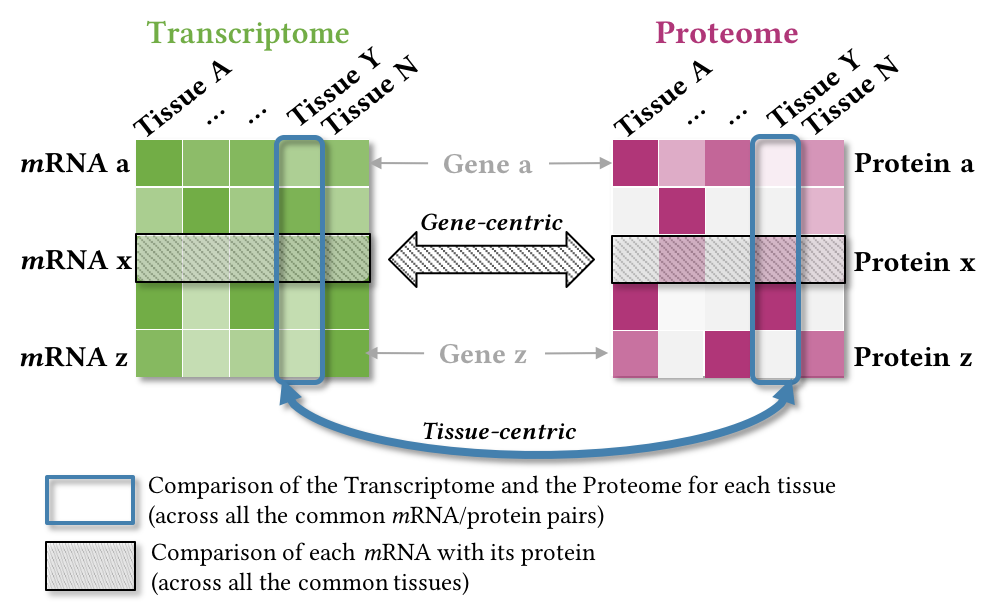
\includegraphics[scale=0.85]{integration/VisualExplaination-Lin.pdf}\centering
    %\vspace{-3mm}
    \caption[Summary of the expression comparison approaches between
    the transcriptome and proteome]{\label{fig:visualexp}\textbf{Approaches
    summary of the expression comparison between the transcriptome and proteome.}
    \emph{Tissue-centric} analyses focus on
    how the transcriptome and proteome relate to each other within the same tissue.
    \emph{Gene-centric} analyses study for each gene how its \mRNA\ expression
    levels across all (or a subset of) the tissues may relate to
    the quantified expression levels of its corresponding protein.
    }
\end{figure}

\Cref{fig:visualexp} summarises the two analytical approaches I use
to compare transcriptomic and proteomic data.
The \emph{tissue-centric} approach compares for each tissue
the global expression of its transcriptomic landscape to its proteomic one.
In contrast,
the \emph{gene-centric} approach compares for each gene
its expression levels in \mRNA\ and protein across all the tissues.
\afterpage{\clearpage\sectionmark{Fair correlations between independent proteomics and transcriptomics}}

Confusion can arise
when integrating proteomics and transcriptomics.
Hence, it is essential
to define the taken approach clearly~\mycite{Liu2016-re}.\mybr\

\section{Fair correlations between independently sourced proteomics~%
and~transcriptomics~of~human~tissues~}\label{subsec:IntegrationGoodCorrProtTrans}
\sectionmark{Fair correlations between independent proteomics and transcriptomics}
\vspace{-2mm}

For the first tissue-centric analysis,
I assess for each tissue the relationship between
the expression of its proteome and transcriptome
through the correlation of the protein expression values
with their corresponding \mRNA\ ones.\mybr\

After scaling with $\log_2(x+1)$,
I compare proteomic and transcriptomic \treps\
from identical and random tissue pairs,
which are similar and roughly correspond to Gaussian distributions
as illustrated by \Cref{fig:distribTrans,fig:pandeyDistribQ1Q2}.\mybr\

\Cref{fig:TestSig} presents the correlation distribution range
of transcriptomic and proteomic \treps\ from identical and random pairs of tissues,
both with Spearman and Pearson correlation methods
(see \Cref{sec:CorrMore}).\mybr\

Although transcriptomics and proteomics have independent sources,
the Spearman correlations of the same tissues \treps\ are equivalent to
correlations in cell studies~\mycite{Lundberg2010-gk,schwanhausserglobal:2011}
where the same sample provides \mRNAs\ and proteins.
Regardless of the protein quantification method
(Top3~\mycite{Silva-Top3} or \PPKM{} ---~\vref{eq:PPKM}),
the median Spearman correlation coefficients are above $0.5$
for matched proteomic and transcriptomic \treps\
(also referred to as \emph{same-tissue pairs}).
The unscaled data presents identical outcomes
(see \Cref{tab:pvalueCorrSP} and \Cref{fig:TestSigUnlog}).\mybr\

The Pearson correlation is closer to the literature
for our new \PPKM\ quantification
than for the Top3 quantification.
The \PPKM\ Pearson correlation averages
above $0.5$ $[$min:~$0.38$~(\Oesophagus)\;; max:~$0.61$~(\Liver)$]$
(and is within $[$min:~$0.45$~(\Oesophagus)\;; max:~$0.67$~(\Liver)$]$
for the untransformed data).\mybr\

\begin{figure}[!htbp]
    \includegraphics[scale=0.8]{integration/DFtestlog2.pdf}\centering
    \vspace{-4mm}
    \caption[Distribution of Pearson and Spearman correlation coefficients
    for same-tissue proteomic and transcriptomic pairs
    versus random tissue pairs]{\label{fig:TestSig}\textbf{Distribution of
    Pearson and Spearman correlation coefficients
    for same-tissue proteomic and transcriptomic pairs versus random tissue
    pairs ($\log_2$-scaled data).} Depending on the protein quantification method,
    there are two types of distribution ranges for the Pearson correlations.
    Top3 quantification method provides a lower correlation ($\text{mean} \approx 0.11$).
    The \PPKM\ method (\Cref{sec:NewQuantProt}) produces higher correlations
    ($\text{mean} \approx 0.5$).
    All the Spearman correlation ranges between same-tissue proteomic and
    transcriptomic \treps\ are quite similar,
    regardless of the method quantifying the proteins.
    The median of Spearman correlation is $0.52$.
    With the Top3 quantification (\ie\ pink countered boxes --- Top3 x HTSeq),
    two outliers are noticeable, and they are common to the three comparisons,
    Pandey x Uhlén (12 tissues and 15 tissues) and Pandey x GTEx (12 tissues):
    the lowest Spearman correlation is \Oesophagus\ ($\rho=0.39$)
    and the highest \liver\ ($\rho=0.62$).
    Both for the Pearson and Spearman correlations,
    even when the correlations are very low,
    same-tissue pairs always have higher correlations than
    different (random) tissues pairs
    (all p-values computed with Welch t-test <0.05 --- see \Cref{tab:pvalueCorrSP}).
    Thus, even the lowest same-tissue correlations are significant.
    The green boxplots, comparing the two transcriptomic datasets,
    are only represented for reference purposes.}
\end{figure}

\begin{figure}[!htbp]
    \includegraphics[scale=0.75]{integration/Kidney_scattplot_Q3_T15.pdf}\centering
    \caption[Scatterplot of protein (Pandey Lab data --- PPKM quantification)
    and mRNA (Uhlén \etal) expression for Kidney]
    {\label{fig:ScatKid}\textbf{Scatterplot of
    protein (Pandey Lab --- PPKM quantification) and mRNAs (Uhlén \textit{et al.})
    expression for Kidney.}
    Each point of this scatterplot represents a gene;
    it has the $\log_2$-transformed expression value
    of the corresponding \uhlen\ \etal\ \mRNA\ (\FPKM) on the x-axis and
    the $\log_2$-transformed expression value of
    the \pandey\ Lab protein (\PPKM) on the y-axis.
    Most of the \mRNA/protein pairs are distributed in an area
    that can be fitted by a linear function with a positive slope,
    which indicates a high correlation between \mRNAs\ and proteins expression
    levels.
    However, genes with lower expressed \mRNAs\ have
    a less associated expression between their protein and \mRNA,
    in particular, \mRNAs\ that are expressed
    below $1$ \FPKM\ (\ie\ below $0$ on the x-axis).
    On the other side, genes with the highest expressed \mRNAs\ may present
    a saturation effect (\Cref{subsec:simpleProt})
    in the quantification of the protein expression.
    The highest expressed protein is \protein{\gls{HBB}}
    (\ie\ Hemoglobin Subunit Beta), which is also found in
    the five highest expressed proteins in all the other tissues.
    Possibly, its presence is due to remaining erythrocytes in the samples.
    On the outer parts of the scatterplot,
    there are the respective distribution densities of the proteins and the \mRNAs.
    Whilst the correlation calculation includes every pair of \mRNA\ and protein,
    the plot excludes any pair with an unexpressed \mRNA\ or protein to optimise the visualisation.
    \Cref{fig:scatplotAll} presents an overview of the other tissue scatterplots.
    }
\end{figure}

As tissue proteomic samples can present high correlation
without being related in any manner
(see \Cref{ch:proteomics,fig:scat2DAdrenalPancreasKuster}),
a Welch t-test~\mycite{Welch1951-sj} allows
assessing the significance of the correlation for the same-tissue pairs
by comparison to random tissue pairs.
The one-sided \Welchttest\footnote{See \Cref{mini:ttest}}
allows rejecting the null hypothesis $H_0$
(the means of the correlation coefficients for same-tissues pairs
are identical or lower to random tissues pairs).
Irrespectively of the protein quantification or computational methods,
all the same-tissue pairs correlations are significant
(p-value $<5.10^{-5}$, except for Pearson correlation with Top3 quantification
where p-value $<0.05$ --- see \Cref{tab:pvalueCorrSP}).\mybr\

The previous correlation distribution
may imply a modest relationship between
these independent proteomics and transcriptomics,
but the same-tissue pairs scatterplots (\eg\ \Cref{fig:ScatKid})
show tighter links than first suggested.
Besides, these scatterplots share a coarse profile
despite the wide correlation ranges.\mybr\

\Cref{fig:ScatKid} illustrates the comparison of expression for \kidney\
between transcriptomics (\uhlen\ \etal) on the x-axis
and proteomics (\pandey\ Lab --- \PPKM) on the y-axis.
\Kidney's correlation coefficients stand in the middle of the range
regardless of the considered studies,
protein quantification or correlation methods involved in the comparison.\mybr\

%To optimise the visualisation,
%I removed the pairs with a null member
%(either for the \mRNA\ or protein)
%while I keep them for the correlation calculation.


A linear function with a positive slope (not drawn) can fit the bulk of the points.
Indeed, the expression of most \mRNAs\ and proteins in a tissue
are highly associated
with the exception of the lowest ($<1$ \FPKM) and
a number of the highest measured \mRNAs{}.\mybr\

Besides the mismatching sampling sources,
other possible explanations for the observed divergences are
technical limitations (such as protein saturation effect, see \Cref{subsec:simpleProt}),
translational noise (see \Cref{subsubsec:exprTrans})
or a consequent half-life difference between the \mRNA\ and its protein.\mybr\

Although the number of genes
presenting lowly associated levels of \mRNA/protein expression is rather limited,
it is enough to impair the Pearson and Spearman correlation coefficients.\mybr\

Systematic exclusion of lowly associated pairs of \mRNAs\ and proteins
is impractical and arguable
as they are inconsistent from one tissue to another.\label{memo:dispersedGenes}
Case-by-case treatment will be necessary.\mybr\

Removing the lowly expressed \mRNAs\ ($<1$ \FPKM) only marginally changes
the correlation coefficients,
\eg\ for \kidney,
when considering the \PPKM\ quantification for the proteins,
the Pearson correlation
increases from $0.56$ to $0.58$,
while the Spearman correlation is relatively unchanged
($0.51$ instead of $0.52$).
There are similar changes observed
when considering the more conservative Top3 protein quantification.
The Pearson correlation $r=0.18$ increases to $0.21$.
The Spearman correlation remains unchanged ($\rho=0.52$).\mybr\

Both transcriptomic studies (\uhlen\ \etal\ or \gtex)
providing equivalent results,
I describe for most of the following analyses the data combination
that provides the greatest number of tissues and genes to study,
\ie\ the fifteen-tissue set between \uhlen\ \etal\ and \pandey\ Lab data
quantified with the \PPKM\ method.\mybr\

\vspace{-1mm}
The other combinations
(provided in \Cref{ch:SupplIntegration} or electronic format)
may diverge for individual genes through the various combinations,
but the general trends are identical.\mybr\
\vspace{-1mm}

I focus on Pearson correlation over Spearman correlation
in the following parts
since the results for the \PPKM\ quantification are globally similar for both.\mybr\

\subsection{Mixed biological signal between the proteome and transcriptome
across the tissues}
%\vspace{-8mm}
\begin{figure}[!hb]
    \includegraphics[scale=0.85]{integration/orderedHeatmapQ3Pearson1.pdf}\centering
    \vspace{-2mm}
    \caption[Heatmap based on the Pearson correlation between protein and mRNAs
    expression (alphabetically ordered tissue)]{\label{fig:orderedHeatmapPearson}%
    \textbf{Heatmap based on the Pearson correlation between protein and mRNAs
    expression (alphabetically ordered tissue).}
    Correlations for same tissue pairs (diagonal) are highlighted in
    yellow when the highest observed correlation are between the matching proteomics
    and transcriptomics pairs; in dark pink, when the proteomics correlates
    the best with the matching transcriptomics.
    When other higher correlations are observed for a tissue proteomics or transcriptomics
    they are in given grey.}
\end{figure}

As shown in \Cref{fig:orderedHeatmapPearson},
for nine tissues (in yellow) transcriptomic and proteomic expressions correlate
better in matching tissues.
For four other tissues (\hColon, \Lung, \Oesophagus\ and \Urinarybladder\
--- in dark pink),
only the proteomics correlate the best with the matching transcriptomics,
while the transcriptomics correlates better with another tissue proteomics.
The remaining two tissues have their proteomics correlating
as much (\eg\ \Gall) to other tissues or more to transcriptomics
from other tissues (\Rectum).\mybr\

While the different correlation methods lead to similar result trends,
individual differences persist.
In a few cases, \eg\ \heart,
these slight differences may change the correlation rank order of
a proteomic \treps\ to the different transcriptomic \treps{}.\mybr\

In the following sections,
I explore several avenues to identify possible factors
that influence the association strength
between the proteome and transcriptome.\mybr\

I first study the effect of tissue composition (in proteins and \mRNAs)
on the correlations.
I begin with the assessment of the impact of the proteins and \mRNAs\
that are found in one tissue only,
before looking into the tissue-specific (\gls{TS}) proteins and \mRNAs{}.\mybr\

Then, in a more quantitative approach,
I examine more closely how the \mRNA\ expression profiles relate
to their respective protein ones.\mybr\

\subsection{Influence of the expression breadth on the tissue %
\texorpdfstring{\MakeLowercase{m}RNAs/proteins}{mRNAs/proteins} correlation}

In \Cref{ch:proteomics},
I have shown that
the protein expression of both different tissues and same-tissue pairs
are sharing a similar correlation range
(see \Cref{fig:scat2DAdrenalPandeyPancreasKuster}).
In this context,
genes expressed in a small number of tissues
(both as a protein and \mRNA)
can have a significant impact on the correlation
and may explain the mitigated results.\mybr\

The expression breadth of a gene is
the number of tissues and cell lines within which the gene is expressed.
\Cref{fig:expressionBreadth} allows visualising
the distribution of the expression breadth of the \mRNAs\ (\uhlen\ \etal)
and the proteins (\pandey\ Lab data) across their fifteen common tissues.
In the following sections,
I can refer to a (\gls{TS}) gene as a \emph{unique gene}
when it is only expressed in a single tissue.\mybr\

\Cref{fig:protBreadth} shows that
the distribution of the protein expression breadth is bimodal.
Either due to technical limitations or biological reasons,
proteins detected in a sole tissue form
the most numerous class and represent 20 \% of the overall number.
Proteins expressed in all tissues are the second most numerous class (about $~$ 16 \%);
the third largest class (12 \%) comprises the proteins expressed in two tissues.\mybr\

On the other hand,
almost all \mRNAs\ are expressed in every tissue (\Cref{fig:mRNAbreadth0}).
One hypothesis is that \mRNAs\ levels have to exceed a sufficient threshold
for their proteins to be detected.
Thus, I also studied the effect of
two additional minimum expression thresholds for the \mRNAs\
on the expression breadth.\mybr\

The two new expression breadth profiles are more alike
to the proteomic one.
As shown in \Cref{fig:mRNAbreadth1},
the number of transcripts only found in one tissue increases
at the widespread $1$ \FPKM\ threshold,
which roughly equates to one \gls{RNA} in the cell~\mycite{Mortazavi2008,Hebenstreit:2011}.\mybr\

The expression breadth profile of the \mRNAs\ expressed at or above $5$ \FPKM\
present a similar bimodal distribution (\Cref{fig:mRNAbreadth5}) to the protein one.
While arbitrary, $5$ \FPKM\ is a threshold commonly found
in the literature~\mycite{Uhlen2015,oneDominant,Chen2018-ln}.\mybr\

\begin{figure}[!htb]
    \begin{subfigure}[h]{0.53\textwidth}
    \captionsetup{margin=0.6cm,justification=centering}
        \centering \includegraphics[width=\textwidth]{integration/breadthProtQ3--15.pdf}
        \caption{Protein~expression~breadth (\PPKM~quantification)}\label{fig:protBreadth}
    \end{subfigure}
    \begin{subfigure}[h]{0.53\textwidth}
    \captionsetup{margin=0.6cm,justification=centering}
        \centering \includegraphics[width=\textwidth]{integration/breadthmRNAQ3--15.pdf}
        \caption{mRNA~expression~breadth\\(> 0 \FPKM)}\label{fig:mRNAbreadth0}
    \end{subfigure}
    \vspace{2.5mm}

    \begin{subfigure}[b]{0.53\textwidth}
    \captionsetup{margin=0.6cm,justification=centering}
        \centering \includegraphics[width=\textwidth]{integration/breadthmRNAQ3--1501.pdf}
        \caption{mRNA~expression~breadth\\(≥1 \FPKM)}\label{fig:mRNAbreadth1}
    \end{subfigure}
    \begin{subfigure}[b]{0.53\textwidth}
    \captionsetup{margin=0.6cm,justification=centering}
        \centering \includegraphics[width=\textwidth]{integration/breadthmRNAQ3--1505.pdf}
        \caption{mRNA~expression~breadth\\(≥5 \FPKM)}\label{fig:mRNAbreadth5}
    \end{subfigure}
    \vspace{-6mm}
    \caption[Expression breadth of the proteins and mRNAs]{\label{fig:expressionBreadth}%
    \textbf{Expression breadth of the proteins and mRNAs.}
    The proteins expression breadth has a bimodal distribution.
    Many proteins are detected either in a single tissue or in all of them.
    Almost every \mRNA\ is detected in every tissue.
    Their breadth becomes bimodal when their expression threshold
    is increased to $5$ \FPKM{}.
    To ease the general visualisation,
    I have omitted to plot the \mRNAs\
    for which the expression remains below the threshold for all tissues
    (\ie\ expression breadth=0 for the considered threshold).
    }
\end{figure}

\Cref{fig:UniqueFeatureQ3T15} displays the fraction of unique genes
(\ie\ only expressed in a single tissue)
detected as a protein or an \mRNA\ at a considered threshold for each tissue as
the analysis is seeking a possible link between
the number of uniquely detected genes
and the correlation strength between the proteomic and transcriptomic \treps{}.
Hence, these fractions are computed by dividing
the number of unique genes (proteins or \mRNAs) of each tissue
by the total amount of uniquely detected genes across all tissues.
The tissues are ordered by increasing order of their fraction.\mybr\

\begin{figure}[!htb]
    \includegraphics[scale=0.78]{integration/uniqueFeatureQ3T15a.pdf}\centering
    \vspace{-5mm}
    \caption[Unique proteins or mRNAs fractions across tissues]{\label{fig:UniqueFeatureQ3T15}
    \textbf{Unique proteins or mRNAs fractions across tissues.}
    }
\end{figure}

Although their proportion varies from one tissue to another,
all fifteen tissues have proteins
that are specifically detected in each tissue solely,
as shown in the top plot in \Cref{fig:UniqueFeatureQ3T15}.
In contrast, unique \mRNAs\ are detected in a more limited number of tissues
(see the three bottom plots of \Cref{fig:UniqueFeatureQ3T15}).
Besides, the unique proteins are more evenly distributed
between the fifteen tissues than the unique \mRNAs.\mybr\

Except for \Testis\ and \Liver,
which are consistently expressing the highest number of uniquely detected genes,
the other tissues fail to present any similarity
between the available proteomic and transcriptomic data.\mybr\

\Liver\ is the most correlated tissue (\Cref{fig:orderedHeatmapPearson})
and comprises the second-highest number of unique genes.
\Testis\ is the third-best correlated tissue
despite having the highest fractions of unique proteins and \mRNAs\
regardless of any threshold.
The other tissues fail to show any relationship
between the unique \mRNAs\ and proteins they expressed
and the strength of the correlations.\mybr\

Put together, these results suggest that
the number of proteins and \mRNAs{} uniquely expressed in these tissues
play a minor role at best in the \mRNA/protein correlation computed for each tissue.
The lack of relation between the proteomic and transcriptomic observations
is confirmed by a more refined analysis of the expression breadth.\mybr\

\begin{figure}[!htb]
    \includegraphics[scale=0.75]{integration/coloredSharedbreadthProtQ3--15.pdf}\centering
    \vspace{-4mm}
    \caption[Comparison of proteins expression breadth to
    corresponding mRNA breadth]{\label{fig:SharedBreadthProtQ3}%
    \textbf{Comparison of proteins expression breadth to their corresponding mRNA.}
    The proteins expression breadth (\Cref{fig:protBreadth})
    is coloured according to
    their corresponding \mRNA\ expression breadth at $5$ \FPKM\
    (\Cref{fig:mRNAbreadth5}).
    About one-fifth of the uniquely detected proteins have
    their corresponding \mRNA\ identically expressed once at or above 5 \FPKM{}.
    The number of proteins classified as \emph{Identical} decreases significantly
    through other breadths until it raises again from thirteen tissues
    to reach about one-third of the ubiquitous proteins.
    Proteins and \mRNAs\ with mismatching expression breadth are split into
    several categories.
    Proteins and \mRNAs\ that are both detected within four to twelve tissues
    are described as \emph{Mixed}.
    If the expression breadths of the remaining pairs are close (± $2$),
    they are identified as \emph{Similar} otherwise as \emph{Different}.
    Finally, many genes detected at least once as a protein have
    an \mRNA\ expression that never reaches $5$ \FPKM{} (\emph{Expression < $5$ \FPKM}).
    }
\end{figure}

\Cref{fig:SharedBreadthProtQ3} shows that the expression breadth
of \mRNAs\ (expressed ≥ $5$ \FPKM\ or even smaller threshold) concurs
in very few cases to their corresponding protein breadth.
Thus, the \mRNA\ expression breadth is insufficient
to predict the expression breadth of the corresponding protein.
Even for the two extreme cases
where the protein is unique to a tissue or ubiquitous (found in all fifteen tissues),
there are differences between the expression breadths of the \mRNA\ and the protein
of the same gene.\mybr\

All the expression breadth analyses of the transcriptome rely on expression levels.
However, \Cref{ch:Transcriptomics} underlines that
high \mRNA\ expression levels are unrelated
to high interstudy correlation of same-tissue pairs
while \gls{TS} \mRNAs\ present a rather strong relation with it.
For this reason, the following analysis examines
the relationship between \gls{TS} \mRNAs\ and \gls{TS} proteins.\mybr\


\subsection{Tissue-specific \texorpdfstring{\MakeLowercase{m}RNAs}{mRNAs} %
have significant overlap with tissue-specific proteins}\label{sec:TSprotMrna}

Unlike \mRNAs,
many proteins are only expressed in one unique tissue.
These are the ones I refer to as \gls{TS} proteins in the remainder of this thesis.\mybr\

To enable the comparison of these \gls{TS} proteins with possible transcript partners,
I first need to define a set of \gls{TS} \mRNAs{}.
To find the latter, I choose the $n$ \mRNAs\ most specific to a tissue
based on the \nameref{subsub:TisSpeGeneMethodPerso} (\Cref{subsub:TisSpeGeneMethodPerso})
where $n$ is the number of \gls{TS} proteins of that tissue.
Then, as detailed in \Cref{fig:RankSpe},
I examine for each tissue the overlap between its $n$ \gls{TS} proteins
with its $n$ \mRNAs\ with the highest tissue-specific ranks.
\Cref{fig:ExJacquard} illustrates the \heart\ example.\mybr\

\begin{figure}[!htb]
    \includegraphics[scale=0.59]{integration/TissueSpeDeter1b.pdf}\centering
    \vspace{-3mm}
    \caption[Determination process of the specific mRNAs]{%
    \label{fig:RankSpe}\textbf{Overview of the comparison of the TS proteins
    and TS mRNAs.}
    \gls{TS} proteins are the $n$ proteins only expressed in one tissue.
    Once the \mRNAs\ have been sorted
    by decreasing order of their relative specificity to a given tissue,
    the first $n$ \mRNAs\ identities are compared
    to the ones of the $n$ \gls{TS} proteins present in the same tissue.
    %Jaccard's similarity coefficients and their significance (p-values)
    %are computed to allow
    %a global assessment of the proteome and transcriptome relationship
    %across all the tissues simultaneously.
    }
\end{figure}

\begin{figure}[!htbp]
\includegraphics[scale=0.63]{integration/overlapRatioPUQ15Q3Heart.pdf}\centering
\vspace{-3mm}
    \caption[Example of overlap of TS proteins and TS mRNAs for Heart]{%
    \label{fig:ExJacquard}\textbf{Example of overlap of \gls{TS} proteins
    and \gls{TS} \mRNAs.}}
\end{figure}

Each tissue has a different number of \gls{TS} proteins.
I thus refine this analysis
by computing Jaccard similarity coefficients
(or Jaccard indices)~\mycite{Jaccard1901-ei,Lin2008-fc},
see \Cref{eq:Jaccard}.
The Jaccard indices allow assessing
the relationship between \gls{TS} proteins and \mRNAs\
across all the tissues at the same time
and ease the result interpretation in contrast to the raw overlap numbers.\mybr\

\begin{minipage}{\textwidth}
    The Jaccard index is computed as follow:
\begin{equation}
    \tag{Jaccard similarity coefficient}\label{eq:Jaccard}
    \begin{split}
        J(x_{1},x_{2}) & = \frac{\left | x_{1}\cap  x_{2}\right |}%
                                {\left | x_{1}\cup  x_{2}\right |}\\
                       & = \frac{\left | x_{1}\cap  x_{2}\right |}%
                                {\left | x_{1} \right | + \left | x_{2} \right |%
                                - \left | x_{1}\cap  x_{2}\right |}\\
    \end{split}
    \raisetag{6cm}
\end{equation}

When applied specifically to \Cref{fig:RankSpe}, we get:
$J(\tikzcircle[Tan,fill={rgb,255:red,195; green,160;blue,153}]{4pt},%
\tikzcircle[DarkOrchid,fill={rgb,255:red,215; green,145; blue,254}]{4pt}) = \frac{k}{2n-k}$,\\
with $n$ the number of proteins (\tikzcircle[Tan,fill={rgb,255:red,195; green,160;blue,153}]{4pt})
that are only found in a given tissue and
$k$ is the number of common genes between \tikzcircle[Tan,fill={rgb,255:red,195; green,160;blue,153}]{4pt}
and \tikzcircle[DarkOrchid,fill={rgb,255:red,215; green,145; blue,254}]{4pt}.
%$n$ most specific \mRNAs\ of the tissue.
\end{minipage}

\vspace{3mm}
To measure the Jaccard indices significance,
I use the hypergeometric test~\mycite{Field2012-au}
(see \Cref{sec:hypergeometricTest}).
In the current analysis,
I consider as success when a \gls{TS} \mRNA\ is among the $n$ \gls{TS} proteins
and test if the number of observed successes is greater than
the expected number for random sampling.\mybr\

\vspace{3mm}
The Jaccard indices for all pairs of the fifteen shared tissues
between the \pandey\ Lab (\PPKM\ quantification) and \uhlen\ \etal\
are summarised in \Cref{fig:JaccardIndexes},
while~\Cref{fig:JaccardPvalues} displays
their respective p-values (hypergeometric test).\mybr\

\begin{figure}[!ht]
    \includegraphics[scale=1]{integration/overlapRatioPUQ15Q3.pdf}\centering
    %\vspace{-3mm}
    \caption[Heatmap of Jaccard indices across 15 tissues]{%
\label{fig:JaccardIndexes}\label{fig:RatioJac}\textbf{Heatmap of Jaccard indices
across the common fifteen tissues between Uhlén \textit{et al.} and Pandey Lab data.}
For each tissue, the \gls{TS} proteins are the proteins
(quantified with \PPKM\ method) that are expressed only in that tissue.
The \gls{TS} \mRNAs\ are the \mRNAs\ with the highest specific coefficients
in that tissue.}
\end{figure}

\begin{figure}[!ht]
    \includegraphics[scale=1]{integration/overlapRatioPvalPUQ15Q3.pdf}\centering
    %\vspace{-3mm}
    \caption[p-values associated with the Jaccard indices]{%
\label{fig:JaccardPvalues}\label{fig:pJacquard}%
    \textbf{p-values associated with the Jaccard indices} of \Cref{fig:JaccardIndexes}.
    These p-values have been computed with the hypergeometric test.}
    \vspace{-3mm}
\end{figure}

%\vspace{4mm}
I have rerun these analyses with different sets of parameters
and I have consistently observed statistically significant overlaps
except in rare cases,
which include the comparison of \gls{TS} genes for \Bladder\
between \pandey\ Lab (\PPKM\ quantification) and \uhlen\ \etal\ (\htseq)
based on the fifteen-tissue set and where the \gls{TS} \mRNAs\ are selected
with the fold change method.
Overall, the Jaccard indices remain within the same ranges
for different sets of parameters.\mybr\

If ranked by their Jaccard indices,
several tissues fall within a range similar to their correlation coefficient,
while other not --- as shown by \Cref{fig:compCorJind}.
For instance, \Liver, \Testis\ and \Pancreas\ have high ranks
and \Bladder\ and \Gallbladder\ low ones
for both their correlation and their Jaccard indices.
On the other hand,
\Kidney\ ranks first for the Jaccard index,
but only reaches the seventh rank for Pearson correlation.
While the \Rectum\ has the smallest Jaccard index
and thus ranks last (\ie\ fifteenth),
it gets ranking number nine for Pearson correlation.
These results suggest that
\gls{TS} proteins and \gls{TS} \mRNAs\ are unrelated to
the tissue correlation levels.\mybr\

%\vspace{4mm}
Overall, the above direct approaches
(based on the gene expression breadth across tissues and their tissue-specificity)
fail to show a prominent (if any) contribution or association
to the correlation levels between the proteome and transcriptome.
These are most likely resulting
from multiple subtle similarities
based on identical differential expression
within many clusters of the proteins and \mRNAs{}.\mybr\

%\vspace{4mm}
Given the unsuccess of direct approaches built on uniquely detected genes,
I next examine whether or not an indirect method may be more appropriate.
For this new analysis,
I build hierarchical cluster trees that try to translate
the tissues' expression \enquote{closeness} or differentiation distances.
Then, I compare the proteins' and transcripts' trees.\mybr\

\FloatBarrier\

\vspace{-8mm}
\subsection{Proteins and mRNAs tissue trees present partial concordant results\quad}
\vspace{-5mm}

As presented in \Cref{subsec:clusteringPres},
a hierarchical clustering analysis requires
a linkage method and
a distance between each element that is included in the analysis.\mybr\

I have built the tree of each dataset by linking the tissues
with Ward's method~\mycite{Ward1963} like in the previous analyses.\mybr\

I have performed an initial analysis that
used the tissue correlations for the distance,
but it did not highlight any similarity
between the proteomics and transcriptomics trees of hierarchical clusters.\mybr\

The distance used in the following analysis reflects
the difference in composition of gene populations expressed by the tissues.
It is based on the Jaccard index (see \Cref{eq:Jaccard}) of the tissues
where I only consider genes (proteins or \mRNAs)
that are detected in two tissues strictly.\mybr\

Making the hypothesis that
the closeness of two tissues increases with the number of genes they share,
I compute the distance between two tissues, $t_1$ and $t_2$
using the following formula:
$\text{distance}(t_1,t_2)= 1 - J(t_{1},t_{2})$.

Note that for this analysis,
I present the results for \pandey\ Lab (\PPKM\ quantification) and \uhlen\ \etal\
for their fifteen shared tissues as for the other analyses,
but I also present and compare with the \gtex\ data and their twelve shared tissues.\mybr\

\Cref{fig:separateTree} shows the hierarchical clustering of the fifteen tissues
for \pandey\ Lab (\PPKM\ quantification)
and \uhlen\ \etal\ (≥ $5$ \FPKM)  studies.\mybr\

%\vspace{-4mm}
\begin{figure}[!htp]
    \begin{subfigure}[b]{0.53\textwidth}
        \captionsetup{margin=0.6cm,justification=centering}
        \centering \includegraphics[width=\textwidth]{integration/TissuePairsQ3T15PandeyJind.pdf}
        \caption{Pandey Lab tissues\\(PPKM quantification)}\label{fig:treePandeyQ3T15}
    \end{subfigure}%
    \begin{subfigure}[b]{0.53\textwidth}
        \captionsetup{margin=0.6cm,justification=centering}
        \centering \includegraphics[width=\textwidth]{integration/TissuePairsQ3T15UhlenCut5Jind.pdf}
        \caption{Uhlén \etal\ tissues\\(≥5 FPKM)}\label{fig:treeUhlenQ3T15cuth5}
    \end{subfigure}
    \vspace{-3mm}
    \caption[Tissues hierachical clustering for Pandey Lab and Uhlén \etal\ data]{\label{fig:separateTree}%
    \textbf{Hierarchical clustering for the fifteen tissues of
    Pandey Lab and Uhlén \textit{et al.} studies.}
    }
\end{figure}

Both \pandey\ Lab and \uhlen\ \etal\ trees,
respectively \Cref{fig:treePandeyQ3T15,fig:treeUhlenQ3T15cuth5}
display the same four pairs of tissues the most closely related:
\Rectum\ and \hColon, \Placenta\ and \Lung, \Liver\ and \Kidney,
and \Testis\ and \Ovary.\mybr\

Comparing more than two hierarchical trees for possible finding congruence
is cumbersome manually;
thus, methods exist to create consensus trees~\mycite{Felsenstein2004-dv}.
The methods can be strict or create a consensus based on the majority.
Since there is a maximum of three trees (one for each dataset)
to compare at a time,
all the consensus trees within this thesis are strict,
\ie\ all the trees must be in agreement on a hierarchical organisation
for the consensus tree to include it.
I use one of the possible implementations of these methods
from the \textbf{\textsf{R}} package
\softCi{ape \normalfont{(v5.2)}}{Paradis2019-ue}.\mybr\

%\vspace{-3mm}
\begin{figure}[!htp]
    \begin{subfigure}[t]{0.53\textwidth}
        \captionsetup{margin=0.6cm}
        \centering \includegraphics[width=\textwidth]{integration/TissuePairsQ3T15Jind.pdf}
        %\vspace{2mm}
        \caption{Consensus tree of the fifteen shared tissues between Pandey Lab
        and Uhlén \etal\ (≥ $5$ FPKM) data}\label{fig:consensus2D15TQ3}
    \end{subfigure}~%
    \begin{subfigure}[t]{0.53\textwidth}
        \captionsetup{margin=0.6cm}
        \centering \includegraphics[width=\textwidth]{integration/TissuePairsQ3T123DFconsensus05Jind.pdf}
        %\vspace{-2mm}
        \caption{Consensus tree of the twelve shared tissues
        between Pandey Lab data and
        Uhlén \etal\ and GTEx data (≥ $5$ FPKM)}\label{fig:consensusTree05}
    \end{subfigure}
    \vspace{-3mm}
    \caption[Tissues hierachical clustering for Pandey Lab and Uhlén \etal\ data]{\label{fig:consensusTrees}%
    \textbf{Consensus of the hierarchical clustering of the tissues across the different studies.}
    }
\end{figure}

\Cref{fig:consensusTrees} shows two consensus trees.
\Cref{fig:consensus2D15TQ3} is the consensus tree built on
the previous trees of \pandey\ Lab and \uhlen\ \etal\ fifteen shared tissues.
The tree groups are clearly featured.
To assay if these groups may still be found beyond these two datasets,
I extend the analysis with the \gtex\ data.\mybr\

\Cref{fig:consensusTree05} relies on the set of twelve shared tissues between
\pandey\ Lab data (quantified by the \PPKM\ method)
and the two transcriptomic datasets (≥ $5$ \FPKM): \uhlen\ \etal\ and \gtex\ data.
Compared to \Cref{fig:consensus2D15TQ3},
only two tissue-sets are consistently observed
as most closely related: \Liver\ and \Kidney, and \Testis\ and \Ovary.\mybr\

Note that the results seem unaffected by the protein quantification method
as \PPKM\ and Top3 methods give identical results.
However, the threshold,
above which the \mRNAs\ are considered,
influences on the analysis' outcomes.
As very few \mRNAs\ are found uniquely in two tissues at $0$ \FPKM,
this threshold is insufficient
to identify any hierarchical organisation in the transcriptomic data.
Increasing the threshold,
for instance to $1$ \FPKM,
allows exposing clusters of tissues, \eg\ \Liver\ and \Kidney{}.

However, different thresholds can also highlight different tissue clusters,
including \Rectum\ and \hColon\ at $5$ \FPKM\
or \Pancreas\ and \Gall{} at $1$ \FPKM{}.
The influence of the thresholds on the results suggests that
genes have their expression levels varying
depending on their tissue context.\mybr\

In summary,
even indirect analyses based on the proteins and \mRNAs\ breadth expression
have some degree of similarity in their results
and seem partially capturing a biological signal.\mybr\

Further more in-depth (direct or indirect) analyses
may clarify the relationship between the proteome and transcriptome.
For example, equivalent correlation levels between specific gene groups
(gene co-expression correlation) may be highlighted
for each tissue at both biological layers.
However, this kind of analyses requiring a case-by-case approach
will greatly benefit from
well-established and proven \mRNA\ and protein expression baselines
for each tissue.\mybr\

The following section \Cref{sec:GenesCorRNAProt} analyses precisely
whether genes have comparable expression profiles
as a protein than as an \mRNA{}.\mybr\
\vspace{-2.5mm}

\section{Wide~correlation~range~for~protein/mRNA~pairs}\label{sec:GenesCorRNAProt}
\vspace{-3mm}
As previously reported, %(on p.~\pageref{memo:dispersedGenes}),
the expression levels of \mRNA/protein pairs can present
a tight relationship in one tissue
while being seemingly unrelated in another.
The first gene-centric analysis explores for each gene
the relationship between the expression levels of its \mRNAs\ and proteins
across all available tissues.
This analysis helps one to determine
whether any intrinsic trend structures the gene expression
or if it is only subject to the environment.\mybr\

\Cref{fig:GeneProtCor} displays the Pearson correlation
between the matching pairs of \mRNAs\ from \uhlen\ \etal\
and the proteins from \pandey\ Lab (quantified with the \PPKM\ method)
across their fifteen common tissues.
The observed levels of correlation (in pink) are higher
than the expected levels computed by random permutation
(the grey line is showing the average of 10,000 permutations).\mybr\

\begin{figure}[!htb]
    \includegraphics[scale=0.9]{integration/PearsonLog2correlationRankedGenes3-15meanPermut.pdf}\centering
    \vspace{-3mm}
    \caption[Pearson correlation coefficients of gene expression levels
    between studies in descending order]%
    {\label{fig:GeneProtCor}\textbf{Pearson correlation of gene expression levels
    between studies across the shared tissues in descending order.}
    For each \mRNA\ and its corresponding protein,
    I have computed their Pearson correlation (in pink)
    across the fifteen common tissue
    between \pandey\ Lab (\PPKM) and \uhlen\ \etal\ data
    and then ordered them in decreasing order.
    The x-axis shows the rank of each pair
    and the y-axis its correlation coefficient
    (computed with $\log_2(\text{level}+1)$).
    The grey line represents the mean of the 10,000 randomisations
    (by pair composition permutation).
    The permutation confirms that the observed correlation coefficients are
    significantly higher than expected by chance.
    The green line serves as the most \emph{ideal} comparison case:
    it represents the Pearson correlation of \mRNAs\ pairs
    between \uhlen\ \etal\ and \gtex\ data.
    }
    \vspace{-1em}
\end{figure}

I also compare the Pearson correlation of the matching \mRNAs/protein pairs
with the ones (in green) of the \mRNAs{}/\mRNAs\ pairs
from \uhlen\ \etal\ and \gtex\ data
to provide more context.
About two-thirds of the genes (8,550) present a strong correlation
($r>0.8$)
between the \mRNA\ expression levels of \uhlen\ \etal\ and \gtex\ data,
but only about 6\% (775) of the \mRNA/proteins pairs are above this limit
(in dark blue).\mybr\

\begin{figure}[!htbp]
    \begin{subfigure}[h]{0.49\textwidth}
        \captionsetup{oneside,margin={0.8cm,0cm},justification=centering,skip=-2pt}
        \centering \includegraphics[width=\textwidth]{integration/antiCorrelated.pdf}
        \caption{Anticorrelated}\label{fig:caseAnticor}
    \end{subfigure}~%
    \begin{subfigure}[h]{0.49\textwidth}
        \captionsetup{oneside,margin={0.8cm,0cm},justification=centering,skip=-2pt}
        \centering \includegraphics[width=\textwidth]{integration/negUnCorrelated.pdf}
        \caption{Uncorrelated}\label{fig:caseUncor}
    \end{subfigure}
    \vspace{1mm}

    \begin{subfigure}[h]{0.49\textwidth}
        \captionsetup{oneside,margin={0.8cm,0cm},justification=centering,skip=-2pt}
        \centering \includegraphics[width=\textwidth]{integration/wellCorrelated.pdf}
        \caption{Well correlated}\label{fig:caseFairlyCor}
    \end{subfigure}~%
    \begin{subfigure}[h]{0.49\textwidth}
        \captionsetup{oneside,margin={0.8cm,0cm},justification=centering,skip=-2pt}
        \centering \includegraphics[width=\textwidth]{integration/HighlyCorrelated.pdf}
        \caption{Highly correlated}\label{fig:caseHighlyCor}
    \end{subfigure}
    \vspace{-2mm}
    \caption[Different cases of correlation for protein/mRNA pairs]%
    {\label{fig:caseGene}\textbf{Different cases of correlation for
    protein/mRNA pairs.}
    The scatterplots show the expression of the genes
    as \mRNA\ in \uhlen\ \etal\ data on the x-axis and
    as a protein in \pandey\ Lab data on the y-axis
    across their common fifteen tissues.
    \Cref{fig:caseAnticor} shows that \gene{SSR3} apparently
    has a protein expression anticorrelated to its \mRNA{}'s one:
    when the \mRNA\ expression is low (\eg\ \Pancreas, \Liver),
    the protein expression is high
    and when the \mRNA\ expression is high (\eg\ \Adrenal, \Prostate),
    the protein expression is low.
    \Cref{fig:caseUncor} features \gene{COL2A1} and for which protein expression
    is observed for many tissues (\eg\ \Oesophagus, \Kidney, \Pancreas)
    while no or very low \mRNA\ expression has been captured.
    \Cref{fig:caseFairlyCor} shows that \gene{TPM2} is expressed in all tissues
    and the expression of the protein is well correlated to the \mRNA{}'s one.
    \Cref{fig:caseHighlyCor} shows that \gene{HGD} has
    highly correlated protein and \mRNA\ expression when found in a tissue.
    Note that true perfect correlation can be observed for pairs
    where both \mRNA\ and protein are tissue-specific (TS).
    }
\end{figure}

The Pearson correlation between the \mRNA/protein pairs ranges rather widely
from $1$ (for 32 pairs,
which are detected as \mRNA\ and protein in the same single tissue only)
to below $-0.5$ (for 105 pairs,
with $r=-0.83$ for the  most anticorrelated one).\mybr\

A closer look at both extremes (\Cref{fig:caseGene})
reveals several possible relationship profiles
between the expression of the \mRNAs\ and proteins.
The negatively correlated genes can present
overall anticorrelated (\Cref{fig:caseAnticor})
or rather unrelated (\Cref{fig:caseUncor}) expression levels
of \mRNAs\ and proteins.
On the other end,
the highest correlated genes present genes
with a tissue-specific (\gls{TS}) protein or
whose \mRNA\ and protein expression levels are tightly related
(\Cref{fig:caseHighlyCor,fig:caseFairlyCor}).\mybr\

\vspace{-4mm}
I only present herein (and in the following sections)
the set of results based on the Pearson correlation of the gene expression levels
between the \pandey\ Lab data quantified with the \PPKM\ method
and \uhlen\ \etal\ data across their fifteen shared tissues
since the different sets share similar results trends.
Furthermore, this data combination provides the highest number of pairs
to be studied across the highest number of tissues.
It also allows continuity with the above tissue-centric analyses.
Complementary results
for Spearman correlation and sets that include \gtex\ data can be found
in digital format at \url{http://www.barzine.net/~mitra/thesis}.\mybr\

%\vspace{-3mm}

\subsection{TS~protein~enrichment~for~the~most~correlated~pairs}
\vspace{-5mm}

\begin{figure}[!ht]
    \includegraphics[scale=0.88]{integration/TSratioBasedOnPearsoncorrelationRankedGenes3-15SimulrowMeans.pdf}\centering
    \vspace{-3mm}
    \caption[TS proteins percentage as a function of
    the considered number of genes (ranked by Pearson correlation)]{\label{fig:Spe_Cor}%
    \textbf{TS proteins percent as a function of the considered
    number of genes (ranked by Pearson correlation).}
    Before being plotted,
    the genes are first ranked in decreasing order of Pearson correlation
    between the expression levels of the two considered datasets
    across their shared tissues.
    The top plot, which is a reproduction of \Cref{fig:GeneProtCor},
    is for interpretive convenience only.
    The two parts of the figure have corresponding x-axes.
    The x-axis of the top plot presents the rank associated with
    the Pearson correlation coefficients of the genes on the y-axis.
    The x-axis of the bottom plot represents
    %opt1
    %the number of genes in the set that includes all the genes up to
    %the considered rank on the top plot.
    %opt2
    the upper limit rank up to which are considered
    the genes (for the calculus).
    The lower limit rank is 1.
    The y-axis of the bottom plot displays the percentage \gls{TS} protein
    for a set of (ordered) genes.
    }
\end{figure}

Here,
I investigate the incidence of the \gls{TS} proteins
on the level of correlation between \mRNAs\ and their proteins.

I first compute for each gene the correlation between the expression levels
of \uhlen\ \etal\ data and \pandey\ Lab data.
Then, I organise the genes in a sequence\footnote{A sequence is an ordered set.}
by ranking them by decreasing order of correlation.
Thus, the first most correlated gene's rank is $1$.
Finally, for each rank $k$ I calculate the number of genes with \gls{TS} proteins
among the first $k$ ranks before converting it into percentage.\mybr\

\Vref{eq:SpeCor} presents the formula with which I compute
the percentage of \gls{TS} proteins.
\Cref{fig:Spe_Cor} illustrates the percentage of \gls{TS} proteins
for a given number of considered genes,
which have been ranked in decreasing order of Pearson correlation coefficients.
Similarly to \Cref{fig:GeneProtCor},
randomised protein/\mRNA\ pairs (average for 10,000 permutations) in grey
and \mRNA/\mRNA\ pairs (\uhlen\ \etal\ data and \gtex\ data) in green
are providing some context.\mybr\

The \gls{TS} protein percentage in pink is extremely high
for the highest range of observed correlation between the expression of
the \pandey\ Lab proteins (quantified with \PPKM) and
\uhlen\ \etal\ \mRNAs\ pairs
across their shared fifteen tissues.
The \gls{TS} protein percentage then decreases quickly
before finally increasing slowly for the lower range of correlation.
Thus, the genes identified as \gls{TS} proteins in \pandey\ Lab data enrich
the most correlated and most anticorrelated \mRNA/protein pairs clearly.
Most of the pairs have a Pearson correlation above 0.5,
although they show a wide range of Pearson correlation,
from $r= -0.77$ (for \gene{ZNF770}) to $r=1$ (for several genes).\mybr\

However,
the corresponding \mRNA/\mRNA\ pairs between \uhlen\ \etal\ and \gtex\ data
show a more evenly distribution of these genes
through the 10, 000 highest gene correlations after an initial peak.
The average of the 10,000 permutations (in grey) of the \pandey\ Lab
with the \uhlen\ \etal\ data also shows
an initial high \gls{TS} protein percentage that drops
to the global amount of \gls{TS} proteins among the complete set of shared genes.
Overall, \gls{TS} proteins represent about one-fifth of all the genes.\mybr\

\subsection{Gene expression profiles clue about biological and technical differences\quad}
\vspace{-6mm}
As mentioned previously,
either artefacts or biology may explain the observed low correlations.
It is rather difficult to identify
which artefacts are specifically impacting each protein/\mRNA\ pair
as there are many and can occur in combination.
However, two major technical sources of artefacts,
which have been reported,
are dispersion for the lowly expressed \mRNAs\ and
saturation for the highly expressed proteins.
See \Cref{sec:transExplo,sec:exploreProtMS} (from p.~\pageref{sec:transExplo})
for more details.\mybr\

\Cref{fig:CorImprovable} shows possible profiles of relationships
between the protein and \mRNA\ pairs.
Well-correlated pairs are in the grey area delimited by the green line.
For these genes, the expression levels of the protein observed in a tissue is
tightly related to the levels of the \mRNA{}.
Although the data have been sampled from different sources,
the stronger associations suggest a similar translation process across the tissues
and may also imply less post-translational modifications
that can hinder protein identification and quantification than for other genes.\mybr\

\begin{figure}[!htb]
    \includegraphics[scale=0.57]{integration/TissueCorInterp}\centering
    \vspace{-3mm}
    \caption[Possible mRNA/protein expression profiles
    due to biological reasons.]{\label{fig:CorImprovable}%
    \textbf{Possible mRNA/protein expression profiles due to biological reasons.}
    Genes with well-correlated transcriptomic and proteomic expression
    are found in the grey area delimited by the green line.
    The genes in the yellow area,
    \ie\ which present a high protein concentration and a low \mRNA\ concentration,
    may have stable proteins and \mRNAs\ with short half-lives.
    The genes in the blue area,
    which present a low protein concentration and high \mRNA\ concentration,
    may have a highly regulated translation,
    a protein challenging to capture with \ms\,
    or a misfit between the annotation definition of their \mRNA\ and protein.
    }
\end{figure}

Genes in the yellow area present a high protein concentration
and low \mRNA\ concentration.
One possible cause may be that these genes have stable proteins
and \mRNAs\ with short half-lives.
On the other hand,
genes in the blue area present a low protein concentration
high \mRNA\ concentration.
These latter genes may have a protein that is more challenging to capture
(either because of unsuited protocols as described in \Cref{sec:exploreProtMS}
or annotation misfits, \eg\ \gene{STAU2} as shown in \Cref{fig:stau2def}),
may forego through higher regulation through their translation
or may be actively exported outside of the tissue that synthesises them.
Anticorrelated genes are another category that will likely require
further analysis for a better overall understanding.
The observed anticorrelation between the proteins and \mRNAs\ expression
can be caused by various elements, which may include
tissue-dependent isomer (either for the \mRNA\ or protein) expression,
self-regulation or a variable secretion rate of the protein.\mybr\

At the time of writing,
the most accurate way to classify the protein/\mRNA\ pairs
remains empirical,
\ie\ human interpretation based on
the joint visualisation of protein and \mRNA\ expression
across the different tissues (and dataset combination).\mybr\

As empirical approaches are better designed
to examine a few genes of interest per study
than to give a broader view of the expression landscape,
in the next section I favour a more general strategy instead.
I study the three gene groups of interest highlighted above
with a \glsdesc{goa}~(see \Cref{sec:enrichmentAnalysis})
to find possible biological factors that may differentiate them.\mybr\

As the pairs with a \gls{TS} protein enrich both the most correlated
and the most anticorrelated genes,
I also choose to study them but separately,
and thus,
I remove them from the most correlated and anticorrelated gene lists.\mybr\

\vspace{-4mm}
\subsection{Distinct functional enrichment profiles
for pairs with a TS protein,
and for the best correlated and most anticorrelated ones}
\vspace{-2mm}

A \glsdesc{goa} (\gls{goa} --- see \Cref{sec:goaGeneralities})
uses gene ontologies that provide defined terms
covering the gene product (\ie\ \mRNA\ and protein) properties.
These terms are structured into categories,
which helps to assess whether a gene set is associated with
a biological process (BP), a molecular function (MF) or a cellular component (CC).
The three ontologies are included
in the \gls{BiocR} package \softCi{org.Hs.eg.db}{orghsegdb}
for analysis in \WebFoCi{\textsf{R}}{https://cran.r-project.org/}{coreR}.\mybr\

The enrichment computation requires
the comparison between the \gls{go} terms set associated
with each studied list of genes to a reference.
I consider three gene lists:
the three hundred best correlated and
the three hundred most anticorrelated protein/\mRNA\ pairs
and all the pairs (2,613) with a \gls{TS} protein.
As a reference, I use the 12, 921 matching protein/\mRNA\ pairs
between \pandey\ Lab (\gls{PPKM} quantification) and \uhlen\ \etal\ data.\mybr\

The \gls{BiocR} package \softCi{clusterProfiler \normalfont{(v3.12)}}{clusterProfiler}
provides a function \textsf{enrichGO},
which implements the \gls{goa} as the over-representation test
described by~\citet{Boyle2004-dh}
and handles all the required statistical testing
and (Benjamini and Hochberg~\mycite{Benjamini1995-nf}) correction.\mybr\

%\begin{landscape}
    \begin{sidewaysfigure}
        \includegraphics[scale=0.95]{integration/goea.pdf}\centering
        \vspace{-3mm}
        \caption[Enriched GO categories for the genes with a TS protein and
        the three hundred with the highest correlations
        and anticorrelationss]{\label{fig:goares}%
        \textbf{Enriched GO categories for the genes with a TS protein,
        the three hundred with the highest correlations and
        the three hundred with the highest anticorrelations.}
        The shared y-axis of the two parts includes the enriched GO categories
        (for any of the three groups).
        The left part of the figure shows
        a heatmap where all the included protein/\mRNA\ pairs (\ie\ 3,213)
        are sorted by their Pearson correlation on the x-axis and
        that each association of a pair with a \gls{go} category is marked.
        The right part shows the results of the BP \gls{goa} analysis
        with \soft{clusterProfiler} (reference: the complete set of 12,921 genes);
        the three groups are showed on the x-axis with their number of genes
        annotated in the considered ontology.
        For each dot, the size represents the ratio of pairs within each group
        contributing to each category enrichment,
        and the colour indicates their significance.
        }
    \end{sidewaysfigure}
%\end{landscape}


The lists of the best correlated pairs and
the ones with a \gls{TS} protein present distinctive enrichment profiles
through the three ontologies.
However, the most anticorrelated pairs list presents
an enrichment only for biological process (BP) terms.
All the individual enrichment \gls{go} analyses
along with the comparison of the enrichment for the CC and MF ontologies
are provided as digital supplementary material.\mybr\

\Cref{fig:goares} presents the results for
the comparison of the enrichment of the three considered gene lists
for the BP ontology.\mybr\

The left side of the figure is a heatmap
that marks the pairs' associations with the \gls{go} categories on the y-axis.
It includes all protein/\mRNA\ pairs of the three studied gene lists.
They are sorted on the x-axis in decreasing order of their Pearson correlation.\mybr\

These \gls{go} categories, shared between both sides of the figure,
combine the five most enriched categories
for each of the three lists (\gls{TS} proteins, best correlated
and most anticorrelated pairs).
The categories enrichment is provided by another \soft{clusterProfiler} function,
\textsf{compareCluster} (which internally invokes \textsf{enrichGO}),
which has also produced the right side plot.
No cross-enrichment of \gls{go} category exists between the three groups
(ensured by the \enquote{\textsf{includeAll=TRUE}} option).\mybr\

Notably, the \gls{go} categories associated with each gene list create
coherent groups of similar biological processes.
The genes with a \gls{TS} protein are enriched in terms for specific signalling,
either for its detection (\enquote{\textit{detection of chemical stimulus}},
\enquote{\textit{sensory perception of chemical stimulus}},
\enquote{\textit{sensory perception}}),
as a response to a signal (\enquote{\textit{G protein-coupled receptor signalling pathway}})
or as a regulation (\enquote{\textit{regulation of signalling receptor activity}}).\mybr\

Concurrently, genes with the best correlated \mRNA\ and protein pairs
of expression are associated with catabolic processes\footnote{%
Catabolic processes are an energy release source
and depend on molecules requiring to be break down~\mycite{molBiolCell}.},
and genes with the most anticorrelated pairs are related to
ribosomes and \glspl{ncRNA} regulation,
thus by extension to the translation and its regulation.\mybr\
%Cellular economics can easily rationalise the modulation
%of the catabolic processes
%with the concentration of their substrates only.
%As for the ribosomes and \glspl{ncRNA} regulation,
%recent studies~\mycite{Xue2015-tf,Genuth2018-az} report that
%they have a more important role than previously expected
%and can modulate the global landscape of expression.
%Isoform variation according to the tissues
%is also more plausible for these genes
%and can contribute as well.
%Furthermore,
%tighter quality controls and more complex maturation process
%may also induce variations in translation rate and yield,
%which may add to the observed differences between tissues.

The \gls{go} terms enrichment analysis with the CC ontology shows
that the best correlated genes are the most enriched
for the following categories:
the \enquote{\textit{postsynaptic membrane}},
\enquote{\textit{apical plasma membrane}},
\enquote{\textit{apical part of cell}},
\enquote{\textit{cluster of actin-based cell projections}},
\enquote{\textit{brush border}}
and the \enquote{\textit{cornfield envelope}}.\mybr\

On the other hand, the pairs presenting a \gls{TS} protein
show a slight enrichment for
\enquote{\textit{ion channel complex}},
\enquote{\textit{transmembrane transporter complex}},
\enquote{\textit{transporter complex}},
and \enquote{\textit{cation channel complex}}.
Whereas the categories associated to the \gls{TS} proteins
are more ubiquitous and can concern every cell type,
the enriched categories for the best correlated genes
are referring more specifically to subsets of cells.
The localisation of the best correlated pairs probably suffers
from their overall ubiquity.
Thus, the results for the best correlated genes are probably an artefact
of annotation
even though they comparatively rely on more genes.\mybr\

The enrichment analysis with the MF ontology
for the best correlated pairs points to different activities:
oxidoreductase, cofactor and transmembrane transporter or signalling activities
(\enquote{\textit{anion transmembrane transporter activity}},
\enquote{\textit{oxidoreductase activity, acting on CH-OH group of donors}},
\enquote{\textit{oxidoreductase activity, acting on the CH-OH group of donors
NAD or NADP as acceptor}},
\enquote{\textit{cofactor binding}},
and \enquote{\textit{coenzyme binding}}).\mybr\

The pairs with a \gls{TS} protein are also associated
transporter and signalling activities
(with the following five categories:
\enquote{\textit{transmembrane singling receptor activity}},
\enquote{\textit{signalling receptor activity}},
\enquote{\textit{molecular transducer activity}},
\enquote{\textit{channel activity}},
and \enquote{\textit{passive transmembrane transporter activity}}).\mybr\

Put together, these results suggest that
when there is a high correlation or anticorrelation between an \mRNA\ and its protein,
biological processes play a more likely role than possible technical confounding.\mybr\

The anticorrelated pairs fail to present any enrichment
for a specific cell compartment or a molecular function.
Thus, it implies that
regardless of their localisation within the cell
or their chemical properties (which relate to their molecular function),
the bottom-up \ms\ studies manage to capture most of the proteins
with variable effectiveness.\mybr\

Nevertheless, bottom-up \ms\ studies favour some proteins,
and missing proteins are a primary source of ambiguities~\mycite{Poverennaya2017-vm}.
Hence, comparing the relative expression levels of proteins within a tissue
may lead to misinterpretations.
On the other hand, while it requires caution,
the relative expression levels of each protein across tissues
ought to provide biological insights.\mybr\

Finally, running all the gene-centric analyses presented above
with the other possible combinations of parameters
mentioned for the tissue-centric analyses
gives similar results.\mybr\

\vspace{-2mm}
\section{Discussion}
\vspace{-2mm}

In this chapter,
I describe the integration and comparison of independent large-scale
proteomic and transcriptomic expression datasets
of undiseased human tissues.
After assessing the range of correlation between the two biological layers,
I have tried to identify possible factors
that may influence the association
between the expression of the \mRNAs\ and proteins.
I have employed both tissue- and gene-centric approaches.\mybr\

Building on insights gained in previous chapters
(particularly \Cref{ch:Transcriptomics,ch:proteomics}),
I have restricted the integration study to
the three following independent sources:
\uhlen\ \etal{}~\mycite{Uhlen2015}
and \gtex~\mycite{GTExTranscript} data for the transcriptomics
and \pandey\ Lab data~\mycite{PandeyData} for the proteomics.
The three datasets share twelve tissues,
while the combined sets based only on \uhlen\ \etal\ and \pandey\ Lab data
present three additional tissues.\mybr\

The above analyses provide
the comparison of \mRNA\ and protein expression across fifteen tissues
for 12, 921 pairs as they include \uhlen\ \etal\ data and \pandey\ Lab data
quantified with our \PPKM\ method (see \Cref{ch:proteomics}).
This new quantification allows encompassing about twice as many proteins
than with the standard state-of-art method (see \Cref{ch:datasets}),
which identifies 6,428 proteins only.\mybr\

The tissue-centric analyses show that
even independently sourced proteomics and transcriptomics of similar tissues
present fair correlation coefficients.
For instance, the range of Spearman correlation
($\rho_{\text{\Oesophagus}}=0.39$
$≤$ $\rho_i$ $≤$ $\rho_{\text{\liver}}=0.62$)
is consistent with the literature,
either published before or during this study (see examples further below).\mybr\

Besides, the new \PPKM\ quantification method for proteins
%introduced in \Cref{ch:proteomics},
provides similar Pearson correlation ranges
($r_{\text{\Oesophagus}}=0.38$ $≤$ $r_i$  $≤$ $r_{\text{\liver}}=0.61$)
to ones previously described for cell studies specifically designed
for the joint integration of \emph{same-sourced} proteomics and transcriptomics
(\eg, \citet{Marguerat2012-sn,schwanhausserglobal:2011,Schwanhausser2013-et,Li2014-ai}).\mybr\

Most remarkably,
all the same-tissue pairs of transcriptomic and proteomic
have a statistically significant correlation
despite the tissue proteomic expression profiles closeness.\mybr\

I have based my following considerations and discussion
on the Pearson correlation results
even though Spearman correlation is often used in the literature
when comparing independent sources of data.
The use of the Spearman method is regularly motivated
by the lack of data distribution normality.
As shown in \Cref{fig:pandeyDistribQ1Q2},
the \PPKM\ quantification produces protein expression levels
that share the same logit-normal profile of distribution
observed for the \mRNAs\ (see \Cref{ch:expression}),
thus allowing an appropriate use of the Pearson method.\mybr\

Next, I have considered several possible properties
that might be factors influencing the mixed correlation levels.
I have compared the expression breadth of the \mRNAs\ and the proteins
before comparing the most specific proteins and \mRNAs\ of each tissue
to one another.\mybr\

The \mRNAs\ and proteins expression breadths
(\ie\ the number of tissues within which an \mRNA\ or protein is expressed)
share the same overall shape for their distribution,
but are only partially concordant.
For example, at 5 \FPKM,
only about 26\% of the proteins that are expressed in one tissue
and about 40\% that are expressed in fifteen tissues have
an \mRNA\ with an identical breadth of expression.\mybr\

The analysis of expression breadth highlights noteworthy facts
--- including a few recently reported in the literature;
\testis\ displays the most unique and diverse expression
both at transcriptomic and proteomic levels
(see also \citet{Wang2019-ut,Zhang2015-yn});
\liver\ (the most correlated tissue) presents the second-highest number
of \mRNAs\ and proteins with a unique expression breadth.
Besides, when the expression breadth of a protein is unique,
the expression breadth of its related \mRNA\ is more likely to be unique
at the threshold of 1 or 5 \FPKM{} as well.
However, the expression breadth of \mRNAs\ gives no indication
of the proteins' one.\mybr\

Nonetheless, \mRNAs{}' and proteins' expression breadths convey
part of the biological signal consistently.
From the Jaccard indices of the proteins and \mRNAs\
solely expressed in two tissues,
I have built hierarchical trees,
and their consensus tree outlines
the \ovary{}/\testis{} and the \kidney{}/\liver{} clusters
at both proteomic and transcriptomic layers.\mybr\

I have then compared the \gls{TS} proteins with the \gls{TS} \mRNAs{}.
The overlaps between the $n$ \gls{TS} proteins (expressed in a single tissue only)
and the $n$ most \gls{TS} \mRNAs\ of each tissue are non-empty,
and except for one tissue (\urinarybladder),
statistically significant with an $\alpha$ level of $0.01$.
While most tissues have similar ranking trends for their overlaps of \gls{TS} genes
and correlation between their proteomics and transcriptomics,
either high levels (\eg\ \liver, \testis\ or \pancreas),
medium (\eg\ \prostate)
or low ones (\urinarybladder, \lung\ or \gallbladder),
other tissues have not.\mybr\

Regarding the gene-centric analyses,
they show that
about $6\%$ of the \mRNAs/proteins are highly correlated ($r≥0.8$),
about $18\%$ of them are well correlated ($0.8 > r ≥ 0.5$),
about $75\%$ of them are poorly correlated ($0.5 > r ≥ -0.5$), and
less than $1\%$ of the pairs are anticorrelated ($-0.5 > r ≥ -0.83$).\mybr\

A fourth of the genes included in this study have a \gls{TS} protein.
Most of them have a Pearson correlation above $0.5$, and
they considerably enrich the set of most correlated pairs of \mRNAs\ and proteins.
However, their correlation range remains rather wide ($-0.77 ≤ r≤ 1$).\mybr\

Finally, using a \gls{go} enrichment analysis,
I have investigated whether the three groups of \mRNA/protein pairs
(the ones with a \gls{TS} protein, the best correlated pairs
and the most anticorrelated ones) are related to
any biological or technical reason.\mybr\

While the most correlated pairs and the ones including a \gls{TS} protein
present an enrichment in biological process (BP),
molecular function (MF) and cellular component (CC) terms,
the anticorrelated pairs present an enrichment only in BP terms.
Overall, the most correlated \mRNA/protein pairs seem highly associated
with catabolic processes;
the pairs with a \gls{TS} protein are most likely involved
with specific signalling (its detection, transduction or answer)
and more concentrated in the transmembrane area.
The most anticorrelated pairs are enriched in regulation processes.\mybr\

On top of the true relationship between the expression of the \mRNAs\ and proteins,
correlations are dependent on the quantification of identified molecules.
In general,
while many biological reasons (\eg\ protein degradation)
can lead to midrange or low correlation levels,
other technical artefacts may also be at play:
saturation effect of more abundant proteins (see \Cref{subsec:simpleProt});
degenerate peptides (see \Cref{subsec:proteinInference});
quantification inconsistencies between methods;
platforms and studies~\mycite{Dapas2017-ui,Aebersold2018-jn};
annotation,
or other oft-neglected sources, \eg\ gene or isoform length.\mybr\

One example where the annotation might be at fault is
\gene{STAU2} (Pearson $r=-0.59$; Spearman $\rho=-0.65$),
which appears to be known to have different annotations
in the proteomic and transcriptomic communities.
Thus, \gene{STAU2}'s anticorrelation observed
between its \mRNA\ and protein expressions
might predominantly result from artefacts
rather than any biological cause.\mybr\

Normalisation methods for \Rnaseq\ require the genes or transcripts length
(see \Cref{subsub:norm}).
To keep congruity with the gene length
employed by \WebFoCi{\egxa}{https://www.ebi.ac.uk/gxa/home/}{EBIgxa},
I use the sum of the lengths of all its collapsed exons,
which is graciously provided by the metapipeline
\softFoCi{\irap}{https://nunofonseca.github.io/irap/}{Fonseca2014-si}.

Although, each gene has various \mRNA\ isoforms~\mycite{MarPhD}
and proteoforms~\mycite{Aebersold2018-jn}
I chose to perform all the analyses at gene-level expression
(see p.~\pageref{minisec:quantNorm})
due to the many existing criticisms about
current algorithms' accuracy with isoforms~\mycite{tamaraRNA,ernestRNA,Dapas2017-ui}.\mybr\

Yet, most genes present one dominant transcript~\mycite{oneDominant}.
One possible method to improve the \mRNA/protein correlations
is to identify the most dominant transcript isoform of each gene
and use their length for the normalisation.
This method ought to be rather easy to implement,
either with the help of resources like
\WebFoCi{APPRIS}{http://appris-tools.org/}{Rodriguez2018-fk}
or through a direct data analysis.
More generally,
besides improving current results,
(even partial) better identification of the \mRNAs\ and proteins isoforms
will most likely unveil still undetected divergences.\mybr\

In terms of the true relationship between the expression of \mRNAs\ and proteins,
it is imperative to remember that the proteome and the transcriptome I use
in the analyses are independently sourced and aggregated over several individuals.
Therefore, some genes displaying mixed correlation in this thesis may present
high correlation or anticorrelation in matched samples.
The most affected genes are the most sensitive ones
to inter-individual variation and batch effects.
On the other hand,
the highly correlated (or anticorrelated) pairs highlighted above
are more likely having a robust expression across individuals and time,
while being less subject to technical noise.\mybr\

Among the studies published during my thesis' works,
three are most notably pertinent to the integration and comparison analyses
I have outlined above.\mybr\

A first published comparison~\mycite{SciRep2016} of the expression data of
\gtex\ \mycite{GTExTranscript} and the \pandey\ Lab~\mycite{PandeyData}
provides weaker results than the above-presented ones
as the authors have based their complete study on data provided as-is
by the primary studies.
Overall, the range of Spearman correlation they present for the tissues
does not exceed $\rho=0.5$.
Additionally, this study also fails to show any functional enrichment
in their selection of matched pairs of \mRNA\ and protein.
Hence, although these primary data resources are useful
for others to appraise the presence of a given gene in a particular tissue,
more thorough uses need more considerations
and probably preliminary treatments.\mybr\

\citet{Franks2017-bp} integrate a subset of the \uhlen\ data included
in this chapter analyses
as they have extracted their transcriptomic data as-is from \citet{Uhlen2014}
to integrate it with the data they have reprocessed
from \pandey\ Lab data~\mycite{PandeyData} and \citet{KusterData}.
The study's primary aim is
to quantify the post-transcriptional regulation of the genes
through their translational efficiency.
To this end, they compute for each gene a \emph{\gls{PTR}}.
\glspl{PTR} ease the assessment of the gene expression variability
across their set of tissues.
This study underlines the utmost caution required
when one considers the transcriptome as a possible proxy for the proteome.
It also reminds that data quality and reliability are primary caveats
for possible analyses.
\citet{Franks2017-bp} also show that genes from the same set of \gls{go} terms
display similar \gls{rPTR} profile across tissues,
\ie\ they have higher and lower \gls{rPTR} in the same tissue sets.
This observation suggests a concerted functionally regulations.\mybr\

Overall, the results presented in this thesis
are confirmed and unsurprisingly improved by~\citet{Wang2019-ut}
since they have matching samples (same sources)
for the proteomics and transcriptomics.
Moreover, there are many biological replicates per tissue.
In that follow-up study, the authors have generated proteomics data\footnote{%
The proteomic data can be retrieved in
\Pride{\href{https://www.ebi.ac.uk/pride/archive/projects/PXD010154/}{PXD010154}}
---\\ \Href{https://www.ebi.ac.uk/pride/archive/projects/PXD010154}}
from the original samples they had used
to produce transcriptomic data\footnote{%
\ArrayExpress{\href{https://www.ebi.ac.uk/arrayexpress/experiments/E-MTAB-2836/}{E-MTAB-2836}}
--- \Href{https://www.ebi.ac.uk/arrayexpress/experiments/E-MTAB-2836/}.}
\mycite{Uhlen2015}, which I am using in this thesis, including this chapter.
While the (Spearman) correlation
between the transcriptome and proteome of each tissue
has a similar range globally,
the expression of an \mRNA\ and its protein across the tissues have
a positive correlation in
about 90\% of all cases and half of them are statistically significant.
They also report that there is
a core set of ubiquitously expressed pairs of \mRNA/protein
and that key differences between tissues are more characterised
by the level of expression of the molecules rather than their presence or absence.
When they compare the highest expressed proteins and \mRNAs,
they observe a limited overlap that, in my opinion,
further confirms that \gls{TS} genes are more pertinent for integration
than the highest expressed genes.
They observed that while disease-associated genes are expressed more globally,
G protein-coupled receptors are mostly restricted to specific tissues,
and are often identified drug targets.
Finally, the authors point out that part of the observed discrepancies
in the proteomic and transcriptomic expression
may be due to the difference in strategies of each community
on how to handle the degenerate peptides or multireads.
Our \PPKM\ quantification presented in \Cref{sec:NewQuantProt}
is one solution to this issue,
and it proves to improve the results,
particularly for the Pearson correlation.\mybr\

A companion study, by \citet{Eraslan2019-md}, reports that
\mRNA\ expression variation across a set of tissues is
a better predictor for protein levels than
considering all \mRNAs\ expression levels in a tissue.
The authors have thus computed a \glsfirst{PTR} for over 11,500 genes.
The study uses these \gls{PTR} to model and probe possible regulatory mechanisms.
However, while \citet{Franks2017-bp}'s \glspl{PTR} may be partially miscalculated
because of the independent sampling sources,
for \citet{Eraslan2019-md}, there might be an overfitting problem.
Further analyses based on other datasets are required
to ensure the reproducibility of these results.
They warn that for many genes,
\glspl{PTR} is only useful as a gauge of the protein abundance magnitude order.\mybr\

Considering the previous papers together with my results,
I have similar correlation levels for same-tissue pairs of
independent proteomics and transcriptomics
to the ones for matched samples (\ie\ collected from the same source)
as I have processed the raw data with consistency.\mybr\

Despite the many deployed efforts,
\eg\ \citet{Franks2017-bp,Eraslan2019-md},
it also seems that predicting protein levels directly from \mRNA\ levels
is still unlikely at the moment.
However, \gls{go} terms may be a useful help in appraising protein expression,
which has been further confirmed in a recent collaboration~$\lbrack$Barzine,
Freivalds, Wright et al. ---\cite{deepLearning2020}$\rbrack$.\mybr\

Additionally, past studies have demonstrated similar results to
the highest correlated pairs of \mRNA/protein
that are enriched with catabolic genes,
and the most anticorrelated ones that are enriched for regulatory processes.\mybr\

\citet{Vogel2010-ux} have observed the highest protein-per-mRNA ratios
for mammalian metabolic genes.
Several papers~\mycite{Vogel2012-sq,schwanhausserglobal:2011}
observe higher expression stability for
\glspl{RNA} and proteins related to mammalian metabolism
and a more rapid degradation tendency
for proteins involved in transcriptional regulation (and chromatin organisation).
Furthermore, organs appear to present
different metabolic profiles~\mycite{Berg2002-vo},
and, regardless of each individual's particulars
(\eg\ sex, alimentary diet, age, physical level),
the expression of many catabolic genes only varies according to the tissue.\mybr\

Accepting the premise that,
regardless of the tissue,
a similar sequence of regulatory steps apply to a gene
(from its transcription to possible post-translational modifications),
taken together the above facts suggest me that
the catabolic genes may have
a more straightforward modulation of their expression than the other genes.
In organic chemistry,
it is well-known that the more a molecule requires steps to be produced,
lesser is its yield (\ie\ final amount).
One possible way to test this hypothesis is to explore if
the amount of substrate can regulated these genes' expression levels.
An indirect approach can be
the comparison across tissues of the co-expression profiles of these catabolic genes
with others involved with the active or passive transport of the molecules
to be degraded (\eg\ transmembrane channel proteins).\mybr\

Another altogether research avenue can be the exploration of possible links
between the tissue-specific (\gls{TS}) genes and the G protein-coupled receptors.\mybr\

\section{Conclusion}

Despite possible batch effects and technical noise,
a part of the biological signal is strong enough
to be consistently captured by the transcriptome and proteome
through direct and indirect analyses.\mybr\

At tissue level,
the independent transcriptomics and proteomics included in these analyses
give similar Spearman or Pearson correlation
to samples produced from same biological sources.
The signal appears stronger for more homogeneous tissues, \eg\ \liver,
or which expression is more distinctive, \eg\ \testis{}.\mybr\

In any cases, a significant number of tissue-specific (\gls{TS}) genes
are consistently shared between proteome and transcriptome.
Besides, even indirect analyses,
such as hierarchical clustering trees
created with genes that are only shared by two tissues,
can highlight identical structures between the two biological layers.\mybr\

On the other hand, the gene-centric analyses have shown that
while only 24\% of the \mRNA/protein pairs are well correlated (r>$0.8$),
most (about 73\%) have a positive correlation for their expression.
While the highest correlated genes are enriched in \gls{TS} proteins,
many of them are expressed ubiquitously.\mybr\

The \gls{go} enrichment analysis on the pairs with a \gls{TS} proteins
highlights that they are enriched for specific signalling,
the most correlated genes are enriched in catabolic processes and
the most anticorrelated ones in regulatory processes.\mybr\

Providing proper care and consistent processing,
one may use these independent resources as part of their study
to achieve lower but still significant results.\mybr\

Results can improve from better identification and quantification alone.
A possible approach can be the standardisation of annotations between communities.
Optimisation or new algorithmic strategies are other ones
as illustrated by our \PPKM\ quantification applied for this thesis' works.\mybr\
